%author : Jérémie VENDRIN, Jérémy CLEMENT


\documentclass[journal, twocolumn]{IEEEtran}
\usepackage[utf8]{inputenc}
\usepackage[T1]{fontenc}
\usepackage{amssymb}
\usepackage{amsmath}
\usepackage[pdftex]{graphicx}

%\usepackage{algorithm2e}
\usepackage{algorithm,algorithmic}

\usepackage[pdftex,bookmarks,colorlinks]{hyperref}
\hypersetup{colorlinks,%
citecolor=black,%
filecolor=black,%
linkcolor=black,%
urlcolor=black,%
pdftex
}


%Pour coller du code dans le rapport
%\usepackage{listings}
%\lstset{language=java,numberstyle=\tiny, breaklines=true}
%\begin{lstlisting}
%\end{lstlisting}

% Définition des différent raccourcis
\newcommand{\frec}{face analysis}
\newcommand{\ii}{\textit{i} }
\newcommand{\nn}{\textit{n} }
\newcommand{\pere}[1]{\textit{$pere_{#1}$} }

\makeatletter
\def\clap#1{\hbox to 0pt{\hss #1\hss}}%
\def\ligne#1{%
\hbox to \hsize{%
\vbox{\centering #1}}}%
\def\haut#1#2#3{%
\hbox to \hsize{%
\rlap{\vtop{\raggedright #1}}%
\hss
\clap{\vtop{\centering #2}}%
\hss
\llap{\vtop{\raggedleft #3}}}}%
\def\bas#1#2#3{%
\hbox to \hsize{%
\rlap{\vbox{\raggedright #1}}%
\hss
\clap{\vbox{\centering #2}}%
\hss
\llap{\vbox{\raggedleft #3}}}}%
\def\maketitle{%
\thispagestyle{empty}\vbox to \vsize{%
\haut{}{\@blurb}{}
\vfill
\vspace{1cm}
\begin{flushleft}
	\usefont{OT1}{ptm}{m}{n}
	\huge \@title
\end{flushleft}
\par
\hrule height 4pt
\par
\begin{flushright}
	\usefont{OT1}{phv}{m}{n}
	\Large \@author
	\par
\end{flushright}
\vspace{1cm}
\vfill
\vfill
\bas{}{\@location, \@date}{}
}%
\cleardoublepage
}
\def\date#1{\def\@date{#1}}
\def\author#1{\def\@author{#1}}
\def\title#1{\def\@title{#1}}
\def\location#1{\def\@location{#1}}
\def\blurb#1{\def\@blurb{#1}}


\date{January 2011}
\title{FACE ANALYSIS}
\author{Jérémy CLEMENT, Jérémie VENDRIN}
\location{Montpellier}
\blurb{%
Université Montpellier 2 --  FMIN319 : INTERACTIVE COMPUTING\\
\textbf{Article presenting research in the field of face analysis}\\[1em]
Supervised by : Stefano Alessandro Cerri
}% 


\begin{document}
\begin{onecolumn}
	\begin{table}[t]
		\centering
  		\begin{tabular}{l c r}
  			
\includegraphics{img/um2.png}& ~~~~~~~~~~~~~~~~~~~~~~~~~~~~~~~~~~~~~~~~~~~~~~~~~~~~~~~~~~~~~~~~~~~~~~~~~~~~~~~~~~~~~&  
\includegraphics{img/um2-1.png} \\
			~~& ~~& ~~\\
			~~& ~~& ~~\\
			~~& ~~& ~~\\
			~~& ~~& ~~\\
			~~& ~~& ~~\\
  		\end{tabular}
	\end{table}

	\maketitle
\end{onecolumn}
\begin{twocolumn}
	\begin{abstract}
		In this paper, we will explain what is the face analysis, today methods, application of this technology, and conclude with futur uses. We based our reflexion on several papers, and web sites about this subject. We think facial recognition is growing and will become an inescapable field of the computers science.

	\end{abstract}

	%Inclure un fichier tex par "section"
	\section{Introduction}
	Since the begining of the computer science, scientists are interested 
about human attitude because of they develop computers with a human model.
That is starting with hardware, wich is organised like human. One 
process unit like brain for human, some extentions like CD or microphone are 
computer's legs and ears.
So, scientists try to give to computers a lots of skills wich are 
comparable to human's skills. A particulary recent skill is the facial 
recognition, a lot of poeple think that will be a futur way for identification, connect with a computer, represent in 3D model people, etc ...


	\section{What is the face analysis?}
	 


	\section{Today methods and application}
	\IEEEPARstart{F}{ace} recognition is a part of biometrics, as well as fingerprints, analysis of hand geometry, iris, retina and voice.
The main application field of biometrics is the access control. It provides solutions safe, cheap, simple and effective.
But in recent years, emerging biometrics in civil matters, for recreational, social and practical purposes.

\subsection{For the access control}

There are two main areas in biometrics : identification and verification.

\paragraph{In the verification or authentication} the biometric system asks the user's identity and tries to answer the question, "Is this person X? ". In an application of the verification system is reliant on biometric information from the user, and compares the data obtained from the characteristic information input with the recorded data corresponding to the asserted identity, it is a one to one comparison (1:1).

The system will find or not find a matching between the two. Verification is commonly used in applications of access control and payment authentication. Biometrics offers many advantages over existing methods of personal authentication such as keys, identification numbers (ID), passwords and swipe cards. Indeed it provided more security and convenience that generates enormous economic benefits and fills the security vulnerabilities of passwords, especially with the current facilities to perform attacks and make cracking.

Thus, these applications are used to identify a large number of people in real time. They are fast and accurate because the reference image has a good quality and image control is taken from the front in optimal conditions.

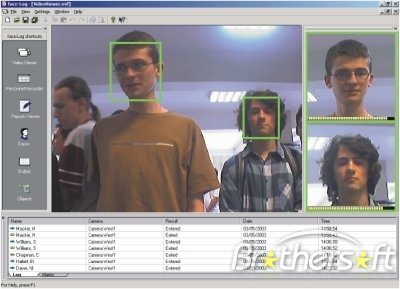
\includegraphics[width=\linewidth]{img/face_recognition_civil}
~\\
Exemples of applications : Passport verification at the airport, windows logon, access to a secure area 

\paragraph{With the identification or recognition} the biometric system asks and attempts to answer the question, "Who is the person X? ". In an identification application, the biometric device requested a biometric information and compares it with every piece of information stored in the database is a comparison to multi (1: N). The object identification applications is to identify criminals and terrorists using the surveillance data.

However, the identification of a suspect filmed by a CCTV camera where conditions are less optimal.
The image is often of poor quality, not always face, facial expression is not neutral, the brightness is different reference pictures.
Again, this time the comparison is not with a single image but with a whole database. The work to be done quickly became much more consistent.

The table~\cite{NPIA} below shows the similarity between the fingerprints searching and the face recognition.

~\\
\begin{tabular}{|p{0.28\linewidth}|p{0.28\linewidth}|p{0.28\linewidth}|}
\hline
\textbf{Fingerprints searching}&\textbf{Face Recognition}&\textbf{Capability}\\
\hline
Ten print to Ten print searching&Mugshot to Mugshot&Identification of an Live Image to Mugshot individual in custody\\
\hline
Ten print to Mark searching&Mugshot to CCTV image&Linking known individuals to unsolved crimes\\
\hline
Mark to Ten print searching&CCTV image to Mugshot&Identifying suspects from forensic evidence at crime scenes\\
\hline
Mark to Mark&CCTV images from multiple cameras&Linking unsolved crimes together\\
\hline
\end{tabular}

~\\

\subsection{Other fields}
\paragraph*{Video Communication and Avatar Chats}
The attractiveness of today's online chat rooms is mainly derived from the secure protection of the anonymity of the chat participants allowing to talk about most private issues if desired. However, the main drawback is the pure text based communication, which lead to an invented chat-language. It comprises numerous different Smileys and *xy* codes for the expression of the emotion, which is so essential for a good communication and fewer misunderstanding.

The protection of anonymity within natural human-human video communication is another application scenario of the FEASy technology. Since the face analysis of FEASy is based on the re-synthesis of a face, the found shapes and positions of eyes, brows, mouth, etc. can be applied to any photography of a face from, say, Brad Pitt, Julia Roberts, or anybody else. Thus, today's text-chat rooms can significantly benefit from providing video chat functionality with the entertainment factor of fitting e.g. celebrities' faces to each chat partner.
\begin{figure}[htpb]
	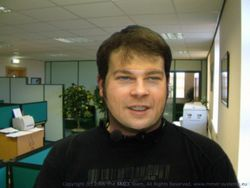
\includegraphics[width=.6\linewidth]{img/avatarchat}
		\caption{Video Communication and Avatar Chats}
\end{figure}

\paragraph*{Facebook}
The social network Facebook announced on Thursday, July 1, the introduction of a new facial recognition system designed to simplify the classification of images published on the site.
"This will probably surprise you, but on the pictures, people take the bulk of their time to download, browse and tag photos. We seek to improve our experience in this field, " says Sam Odio, head of Facebook on the official blog of the group.
The aim of the new device is indeed simplify the identification of these images. On each photograph, when a face is recognized automatically by the program, a window appears asking the user's social network to include the full name of the person, or any other keyword. Two months ago, the company had already acquired the sapling Divvyshot specializing in facial recognition.
\cite{facebook}

\paragraph*{NeoFace}
The solution NeoFace Nec, equips the Hong Kong Immigration Department, by matching the number plate with the driver's face, correspondence established at the time of passport application and the barrier at the border opens.

\paragraph*{Targeted messages on billboard}
Companies like Quividi offer targeted messages solutions depending on the person viewing the billboard. The idea:
\begin{itemize}
\item You're a teenager with lots of button -> Biactol
\item You're a mom with a stroller -> Guigoz
\item A couple held hands - no alliance -> Pronuptia
\item A little old man with a cane -> Aviva, for a convention of funeral
\end{itemize}

\paragraph*{Facelook}
Polar Rose, a Swedish company just purchased by Apple, moved to link different profiles (facebook, lastfm, twitter,...) to your face from your mobile phone.

You're on a beach in Barcelona.
A girl you like, you would like to know more about her.
You installed the application on your mobile, you point to the girl.
Face recognition allows you to find your profile.
A modern version of the sweeper.
\begin{figure}[htpb]
	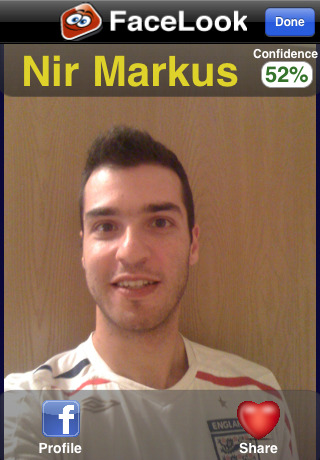
\includegraphics[width=.6\linewidth]{img/facelook}
		\caption{Video Communication and Avatar Chats}
\end{figure}

\paragraph*{FaceAPI}
faceAPI allows you to incorporate Seeing Machines world class face tracking technology into your own product or application. faceAPI provides a suite of image-processing modules created specifically for tracking and understanding faces and facial features. These powerful tracking modules are combined into a complete API toolkit that delivers a rich stream of information that you can incorporate into your own products or services. Seeing Machines faceAPI is the only comprehensive, integrated solution for developing products that leverage real-time face tracking. All image-processing for face tracking is handled internally, removing the need for any computer vision experience.

\begin{figure}[htpb]
		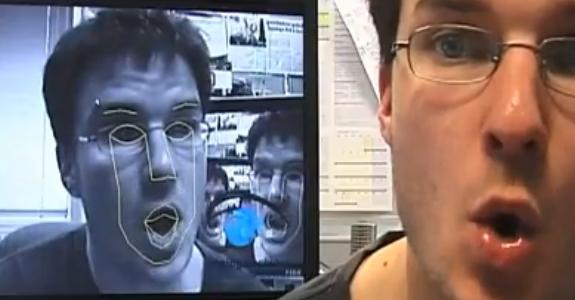
\includegraphics[width=.6\linewidth]{img/faceapi}
		\caption{FaceAPI}
\end{figure}


	\section{Today researchs for tomorow uses}
	\IEEEPARstart{N}{owadays} searches look at facial features detection, and facial expression recognition. Indeed, for analyse a face there is several methods. Principal Component Analysis (PCA), Linear Discriminant Analysis (LDA), and Independent Component Analysis (ICA) are most used methods \cite{Using-Graph}\cite{active-appearance-model}.In this part, we will quickly present each typical methods employed for analyse a face. These approchs are not used alone, they are often combinated\cite{Two-Dimensional}\cite{Active-Shape}.\\
	
	
	\subsection{Principal Component Analysis (PCA)} \leavevmode\par
	PCA\cite{PCA} is a useful statistical technique that has found application in fields such as face recognition and image compression, and is a common technique for finding patterns in data of high dimension. For use PCA, we need to have several images available. PCA represent images such as this :
		\begin{itemize}
		\item For an image I (nxn), there is $n^{2}$ pixels.
		\item For k images PCA extract $n^{2}$ k-dimensional vectors.	
		\item After that PCA reduce vector space dimension. The result of the five step of PCA give us a simple way to know if two images are neighbor.
		\end{itemize}
	
	Now we have an average image, wich is a concept. If we use a learning method, for create an average face with each basic images. With all of these average faces, we create a covariance matrix. Now we can calculate eigenfaces and we project base's visages in eigenfaces' subspace.
	And to finish compare Euclid distance of images.
		
		
	\subsection{Linear Discriminant Analysis (LDA)}
	The linear discriminant analysis (LDA) is used to find the linear combination of features that is the best separation between
object classes or events. The resulting combinations can be used
as a linear classifier, or generally in reducing characteristics before
subsequent classification.
LDA is closely related to PCA, because both seek combinations
combinations of variables that best represent the data. LDA explicitly attempts
modeling the difference between classes of data. PCA to when it does not take into account
differences between classes.
Every face, which consists of a large number of pixels is reduced to a smaller
set of linear combinations before classification.
Each of the new dimensions is a linear combination of pixel values, which
form a template. The linear combinations obtained using FLD called
Fisherfaces, in analogy with the Eigenface.
LDA is a technique that seeks directions that are efficient for discrimination
between data.
LDA is known for its rather maximizing inter-class scatter and minimizing the intra-class scatter, which is manifested by the group of weight vectors of the same class (small distance between these vectors), and the separation of weight vectors of different classes
(large distance between these vectors).
\begin{figure}[h]
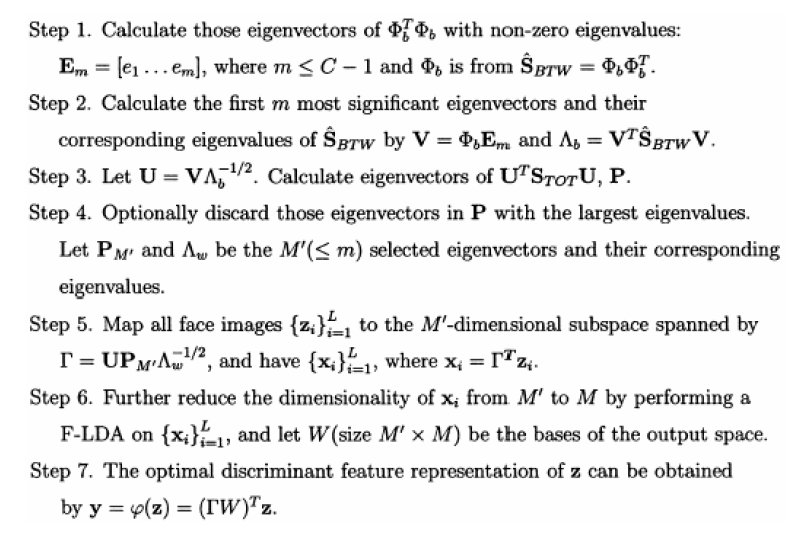
\includegraphics[width=\columnwidth]{img/step.png}
\caption{The algorithme - LDA}
\end{figure}

\subsection{Independent Component Analysis (ICA)}
	PCA is an optimal technique to search a reduced representation that minimizes error
reconstruction, the basis vectors taking into account the reconstruction error
may not be optimal for encoding information appropriate to the image
classification. The independent component analysis ICA is a generalization of PCA, the higher order statistics, which can
produce a more powerful data representation.
The goal of ICA is to find basis vectors localized in space and are statistically independent, minimizing the statistical dependence.


\subsection{Learning Vector Quantization (LVQ)}
The application of artificial neural networks in face recognition is for solve several problems face recognition and
classification of facial expressions.
A neural network is a system of information processing that was developed
as generalizations of mathematical models matching human knowledge. They
consist of interconnected processing units called neurons,
working together for perform a given task.
A neural network is a distributed parallel work. It resembles the human brain in three
aspects: knowledge is acquired by the network through a learning process, strengths
connection connected together, and each neuron has an internal state called threshold or function
activation used to classify the vectors.

A classification by neural network comprises the following steps:
\begin{itemize}
\item First a pre-learning image processing and association with each learning image (network input) an output vector, then comes the stage initialization (creation of network layers). 
\item It makes learning (supervised) in the network,
until it reaches a certain minimal error (the network learns to classify the images well
learning). 
\item We then present a new image to the network to identify (phase
recognition or activation or simulation of the network) that is ultimately assigned to a
given class . 
\end{itemize}

\subsection{Template matching}
The template matching technique is a global face recognition\cite{Image-Based}. The correlation
is generally used to measure the similarity between a template wich is a mask and stored
image to recognize. The templates should be deliberately designed to cover the variety
possible variations of the image.
While searching in the image, scale and rotation should also be
carefully considered to accelerate the process.
This technique was also used to locate the salient features "salient
features "such as eyes nose and mouth in a face image.

The template matching algorithm:
\begin{itemize}
\item Acquisition, reading and standardization of training images.
\item Calculates the average face of each class of persons (templates).
\item Acquired the reading and the normalization of the image audit.
\item Calculates the differences between the verification image and the template (the differences are images).
Is calculated based on amount of these differences (sum of pixel image difference).
\item And finally the minimum amount which will reference the class belongs image verification.
\end{itemize}

\subsection{characteristic points method}
\subsubsection{Cross ratio}[h]
	\begin{figure}
	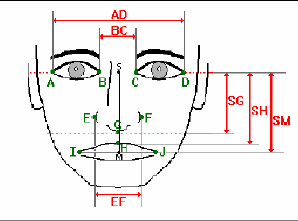
\includegraphics[width = \columnwidth]{img/ratio.png}
	\caption{Face ratios}
	\end{figure}
	The first local recognition methods were based on the width of the head, and
the distances between the eyes and mouth, by calculating the relationship between these distances. These methods are easily affected by irrelevant information.
The recognition algorithm using the Cross Ratio:
\begin{itemize}
\item Extraction of facial characteristic points (affected by the orientation of the head).
\item Definition of Cross Ratio for each 4 points of a line (distances
invariable). 
\item Make the correction of the location of characteristic points by
the application of symmetry and the cross ratio. 
\item Normalize after the feature vector:
N = F / | | F | |
\item And finally we use the Euclidean distance as a similarity measure.
\end{itemize}


\subsubsection{Elastic Graph Matching}
	\begin{figure}[h]
	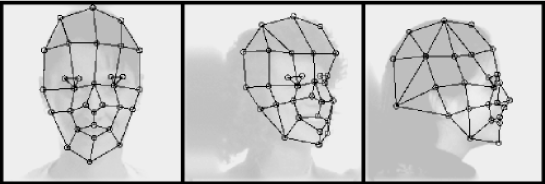
\includegraphics[width = \columnwidth]{img/egm.png}
	\caption{Elastic Graph Representation}
	\end{figure}
	The algorithm EGM "Elastic Graph Matching" represents individual faces a rectangular graph. Each node
	graph labeled with a set of complex coefficients of the Gabor wavelets
	called jets different orientations and scales. A jet is used to represent
	 face images based on wavelet transform
	Gabor. Only the magnitudes of coefficients are used for recognition.

	To recognize a new face, each graph of the database is adjusted to
	this new graph constructed, and the good fit indicates the recognized person.
	Initial results obtained encourage the use of faces with wide rotation
	angles. DLA is generally good in terms of variation of rotation, however,
	recognition process or adjustment is costly in computation.
	The EGM uses the phase of the complex coefficients of Gabor wavelets to achieve a
	more precise localization of the nodes and to differentiate between similar models in their
	coefficients of magnitude.
	The use of graphs EGM adaptive object "Adaptive object graphs," whose nodes
	referring to specific facial landmarks, or fiducial points "fiducial points" in
	face, namely the pupils, the corners of the mouth and nose.

\subsection{So ...}
We can see that the domain of researches in face recognition is very large. In each of these method, searchers work hard to find more an more best methods. A lot of team around the world are working about this subject.
	
		




	\section*{Conclusion}
	\IEEEPARstart{T}{o} conclude, we can say face recognation is expanding. We have got currently some systems which implement some simple features. We don't finished research in this area, we can see that in all cited articles. This domain is a new way for interactive computing, that make available face interactions with computers. We can imagine invalid people wich can communicate with others across computer analysing her face. It's like fantasy books, systems can percept our emotions, so can analyse them. Interact our houses, an emote reacting house wich don't open lights to strong if you aren't awake. A car can start cooling because of it see you perspiring...\\
One question come on our mind, twisted with other technologies like robot, and artificial intelligence system, is that giving to machins skills which will make them more and more humans?\\


	\cite{NPIA}
	\cite{nyuLucasHelen}

	\bibliographystyle{plain}
	\bibliography{biblio}

\end{twocolumn}
\end{document}
